\chapter{Som}
\label{chap.som}

Os módulos ligados ao processamento e geração de ficheiros de som seguiram os moldes do que foi sugerido no enunciado do projeto. Foi criado um interpretador de pautas, um sintetizador e um processador de efeitos. Criámos também um método para a criação de imagens com a representação das notas das músicas.

\section{Interpretador de pautas}

O interpretador recebe uma pauta no formato \ac{rtttl} e devolve uma lista de pares duração-frequência, cada par correspondendo à nota e sua respetiva duração. Tomemos como exemplo a seguinte pauta:

\vspace{5mm}
\textbf{"Barbie girl : d=4, o=5, b=125 : 8g\#, 8e, 8g\#, 8c\#6, a, p, 8f\#, 8d\#, 8f\#, 8b, g\#, 8f\#, 8e, p, 8e, 8c\#, f\#, c\#, p, 8f\#, 8e, g\#, f\#'}
\vspace{5mm}

Neste caso, o interpretador devolve uma lista com 23 pares, com a seguinte estrutura:

\vspace{5mm}
\begin{lstlisting}
[{'freq': 830, 'time': 0.24}, {'freq': 659, 'time': 0.24}, {'freq': 830, 'time': 0.24}, {'freq': 1108, 'time': 0.24} ... ]
\end{lstlisting}
\vspace{5mm}

Internamente, o interpretador começa por ignorar a primeira parte da pauta, correspondente ao nome. De seguida, analisa os valores dos parâmetros de referência, d, o e b. Caso algum não esteja definido, é aplicado o valor padrão (d=4, o=6 e b=63). Por fim, extrai a parte correspondente às notas e percorre nota a nota, tendo a vírgula como referência para as separar. Para determinar a frequência da nota para uma dada oitava, foi criada uma \emph{lookup table}, sendo devolvida a frequência quando é inserido como parâmetro a seguinte expressão: [12 * oitava + tom] - com a oitava a variar entre 0 e 7 e o tom entre 0 e 11. O 0 correspondente ao dó e o 11 ao si. No final do cálculo da frequência e tempo de cada nota, o par é adicionado à lista, que no final é devolvida.

\section{Sintetizador}
O sintetizador recebe como argumentos os pares vindos do interpretador e um registo, devolvendo uma nova lista com a frequência (principal) e respetivas amostras ao processador de efeitos. Inicialmente são criadas as seguintes variáveis:

\begin{itemize}
\item sounds - lista vazia, que irá ser a devolvida no final;
\item freqs - lista de tamanho 9, que irá conter os 9 frequências para cada nota;
\item ratio - lista de tamanho 9 com os múltiplos para o cálculo das 9 frequências para cada nota, de acordo com os osciladores: [1/2, 2/3, 1, 2, 3, 4, 5, 6, 8];
\item amplitudes - lista de tamanho 9 que irá conter as amplitudes das frequências para cada nota, de acordo com os valores definidos no registo.
\item rate - inteiro para a frequência de amostragem, que é sempre 44100.
\end{itemize}

De seguida, o sintetizador percorre a lista de pares recebido do interpretador, alterando a lista de frequências para cada nota. Produz as amostras com a duração definida, correspondendo à soma das 9 componentes sinusoidais. Estas têm a amplitude e frequência previamente calculadas e guardadas nas listas referidas acima. No final de cada nota ser processada, a frequência principal e amostras são adicionadas à lista sounds, devolvida no final. A lista fica com a seguinte estrutura:

\vspace{5mm}
\begin{lstlisting}
[{"freq": 830, "samples": [0, 11775, 18804, 19193, 14747, 9339, ...], {"freq": 659, "samples": [...], ...]
\end{lstlisting}
\vspace{5mm}

Os cuidados com a possível existência de \emph{clipping} não são tomados nesta altura, pelo ue existirá um método para normalizar as amostras mais à frente, no processador de efeitos.

\section{Processador de efeitos}
O processador de efeitos recebe a lista de sons vinda do sintetizador e o efeito pretendido, tendo como função gerar o ficheiro de som da música. Nas secções seguintes irá ser explicado como é aplicado cada um dos efeitos.

Depois do efeito pretendido ser aplicado, as amostras são normalizadas, para poderem estar contidas no intervalo de resolução (-32768 to 32767), sendo posteriormente empacotadas e utilizadas na geração do ficheiro wav.

\subsection{Efeito nulo}
A partir da lista de sons fornecida, extrai a lista de amostras de cada som e junta-os numa única lista, para poder devolvê-la no final.

\subsection{Efeito eco}
Aplica inicialmente o efeito nulo e, seguidamente, percorre a lista de amostras, somando a cada uma um múltiplo (inferior a 1, para atenuar) da amostra correspondente a 0,1 segundos atrás e outro múltiplo (inferior ao anterior, para atenuar ainda mais, pois é um eco mais atrasado) da amostra 0,2 segundos atrás. Deste modo, são introduzidos dois ecos, com atrasos de 0,1 e 0,2 segundos.

\subsection{Efeito trémulo}
Aplica inicialmente o efeito nulo e, seguidamente, percorre a lista de amostras, adicionando a cada amostra uma outra amostra de uma sinusoidal de frequência 20Hz. O resultado é uma música com oscilações rápidas de amplitude, dando a ideia de vibração.

\subsection{Efeito distorção}
Aplica inicialmente o efeito nulo e, seguidamente, percorre a lista de amostras, elevando ao quadrado cada amostra.

\subsection{Efeito percussão}
Tem como objetivo de no início da música ou depois de uma pausa sobrepor uma harmónica, que se vai anulando ao longo do tempo. Para tal, começa por aplicar no primeiro conjunto de amostras essa harmónica (início da música) e, para as notas seguintes, volta a aplicar uma harmónica, caso a frequência principal das amostras da nota imediatamente anterior seja zero (pausa).

A modulação da amplitude de cada harmónica ao longo do tempo é baseada numa lista previamente criada (ver \autoref{percussionlist}), na qual se pode aceder a um índice entre 0 e 200. Para cada índice, vem um múltiplo (entre 0 e 1) pelo qual se deve multiplicar a amplitude da onda.

\begin{figure}[htp]
\centering
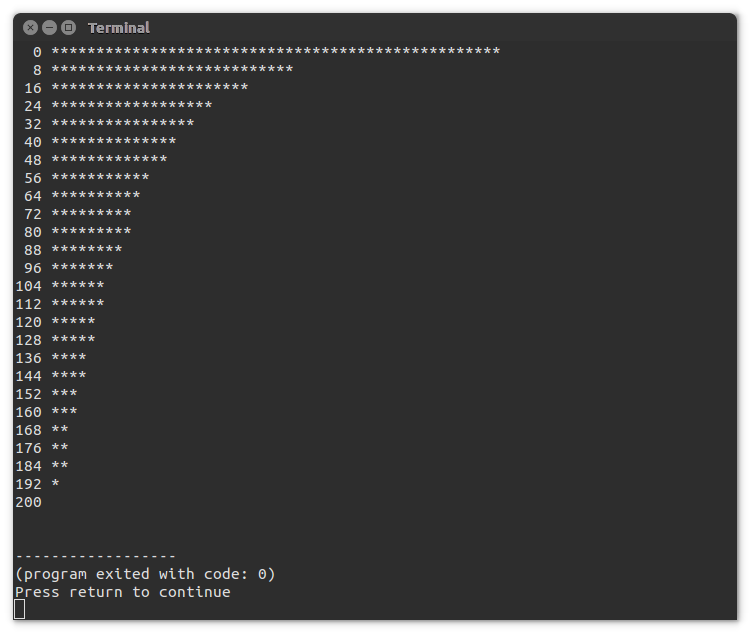
\includegraphics[width=\textwidth]{images/percussionlist.png}
\caption{Visualização gráfica através do terminal dos valores da lista utilizada para calcular os múltiplos da amplitude da onda no efeito percussão. No repositório, pode executar-se o ficheiro som/decreasing\_list\_test.py.}
\label{percussionlist}
\end{figure}

\subsection{Efeito coro}
Para cada nota, percorre a lista de amostras, adicionando 3 sinusoidais com +20, +30 e +50 Hz que a frequência principal, tendo como efeito um conjunto de sons de fundo que acompanham a música principal.

\subsection{Efeito envelope}
Para cada nota, percorre a lista de amostras, moldando a amplitude total da nota de acordo com uma lista previamente criada (ver \autoref{envelopelist}), na qual se pode aceder a um índice entre 0 e 200. Para cada índice, vem um múltiplo (entre 0 e 1) pelo qual se deve multiplicar a amostra.

\begin{figure}[htp]
\centering
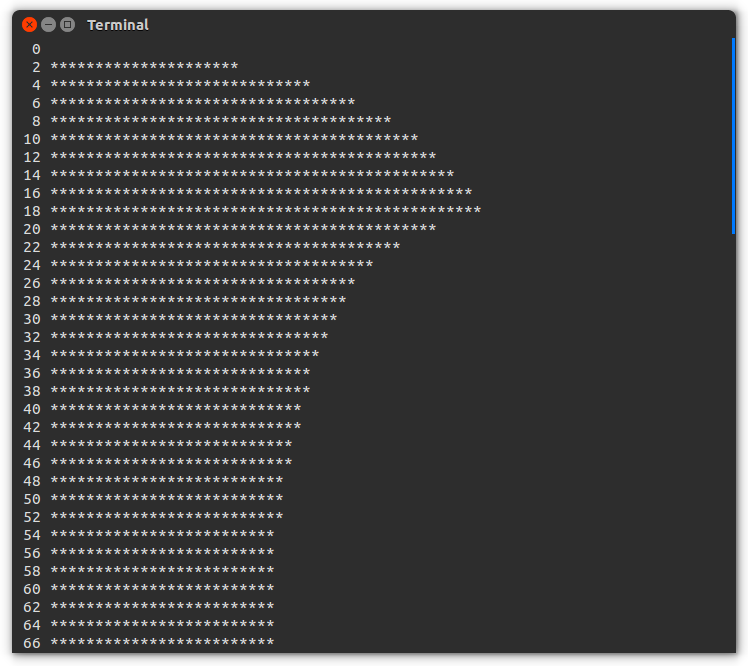
\includegraphics[width=\textwidth]{images/envelopelist.png}
\caption{Visualização gráfica através do terminal dos primeiros valores da lista utilizada para calcular os múltiplos da amplitude das amostras no efeito envelope. No repositório, pode executar-se o ficheiro som/envelope\_list\_test.py.}
\label{envelopelist}
\end{figure}

\section{Imagem da Pauta}
O método que cria as imagens chama-se create\_image e recebe como argumento os pares vindos do interpretador e uma string com indicação do nome pretendido para o ficheiro.

Para tal, é utilizada a biblioteca PIL \cite{pil}, que tem a utilidade de gerar o ficheiro JPEG final.

O método começa por criar uma nova imagem toda a branco, com dimensões calculadas a partir do número de notas e do espetro de frequências possíveis. Foi escolhido o modo de representação de cor \ac{bw}, visto pretender-se escrever as notas a preto em fundo branco. Deste modo, a imagem gerada fica também um pouco mais leve.

Seguidamente, o método percorre a lista de pares. O posicionamento da nota na imagem é calculado baseando-se na frequência, para a altura, e na duração, para o comprimento. São alterados para preto os pixeis correspondentes à zona onde a nota deve ficar desenhada. Caso a nota seja uma pausa (frequência zero), esta não é representada, visto tratar-se de uma pausa.

No final do processo a imagem é recortada, dado que na maioria das vezes o espetro de frequências e, por consequência, a altura da imagem, nunca é utilizada na sua totalidade. O resultado final pode ser observado na \autoref{thesimpsons}, que representa as notas da música The Simpsons.

\begin{figure}[htp]
\centering
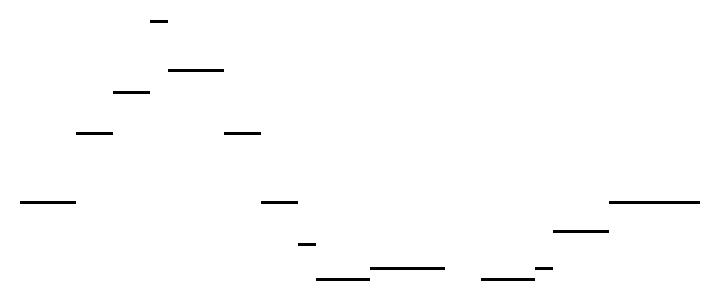
\includegraphics[width=\textwidth]{images/thesimpsons.jpg}
\caption{Visualização gráfica das notas feita a partir da música The Simpsons.}
\label{thesimpsons}
\end{figure}
